% =========================================================================
% CHAPTER 5
% =========================================================================

\chapter{Software Design}
\label{K5}
\section{Deployment}
\begin{wrapfigure}{r}{0.275\textwidth}
  \vspace{-24pt}
  \begin{center}
    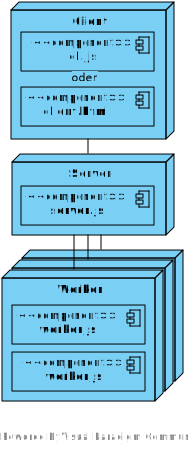
\includegraphics[width=0.275\textwidth]{deploy}
    \caption{UML Deployment Struktur mit Netzwerk Verbindungen. Client ist entweder CLI-Client oder
     Webclient.}
    \label{fig:deploy}
  \end{center}
  \vspace{-50pt}
\end{wrapfigure}

Die Implementierung besteht aus mehreren ausführbaren Komponenten: ein CLI-Client, Webclient, dem Server und den Workern (siehe Abbildung \ref{fig:deploy}).
Im Folgenden werden Instanzen dieser als Node bezeichnet.
Bis auf den Webclient sind sie alle als Node.js Script ausgeführt.

Die Unterschiede dieser Komponenten sind gering.
CLI-Client und Webclient unterscheiden sich von den anderen Komponenten nur durch das zusätzlich enthaltene UI.
Die Worker unterscheiden sich vom Server nur dadurch, dass sie ClientWebSockets anstatt ServerWebsockts verwenden.
Dieses Design wurde gewählt, um zukünfigte arbeiten mit P2P und HCSNO mit mehreren Worker Ebenen zu erleichtern.

Ansonsten hat jede dieser ausführbaren Komponenten intern den gleichen Aufbau, welcher in den folgenden Abschnitten beschrieben wird.




\section{NetInfo}
Als ein globales Objekt ausgeführt, steht diese Komponente in allen Modulen zur Verfügung, auch in JobScripts.
Verwendung findet sie vor allem in JobScripts, um geeignete Worker auszuwählen.
Das NetInfo Objekt besteht aus einer Liste der im System vorhandenen Nodes.
Jede Node darin bietet folgende Eigenschaften:
\BCL
  \setlength\itemsep{0.0em}
  \item Funktionen zum Empfangen und Senden von Daten
  \item Momentane CPU- und Speicherauslastung
  \item Informationen über das Betriebssystem
  \item Liste der auf dem Gerät installierten Interpreter
\ECL
\noindent Um CPU- und Speicherauslastung aktuell zu halten, senden alle Teilnehmer zyklisch Updates an den Server.
Dieser leitet sie an die Clients weiter.
Derzeit ist noch keine Publish-Subsribe Implementierung vorhanden, sollte aber verwendet werden, um die Netzwerkauslastung zu minimieren.
Die Struktur des Network Overlays ist durch Konfiguration definiert, Clients und Worker verbinden sich mit dem Server, wodurch ein HCSNO entsteht.




\section{App}
Eingehende Nachrichten werden an das App Modul weiter gegeben.
Zunächst ist es dessen Aufgabe, den zur Nachricht gehörenden Job zu finden, beziehungsweise einen neuen zu erstellen falls es eine Call Nachricht ist.
Wie in Kapitel \ref{K4} beschrieben, enthalten die Nachrichten JavaScript Code, welcher vom App Modul in einer Sandbox ausgeführt wird.
Innerhalb dieser Sandbox stehen der Job, das NetInfo Objekt, die Job- und Tooljob-Implementierungen zur Verfügung.




\section{Job Interface}
\label{JobInterface}
Die abstrakte Job Klasse implementiert die in Kapitel \ref{jfsm} beschriebenen State Machine.
State Transitions werden mit den Funktionen call, cancel, update und return ausgelöst.
Die Implementierung der Job Klasse ist verantwortlich für das Abfangen von nicht erlaubten Transitions und für Timeouts.
Sie führt die abstrakten Funktionen onCall, onCancel, onUpdate, onReturn zur jeweiligen Transition aus.
Die Implementierungen  dieser Funktionen werden im Konstruktor übergeben.

onCall muss definiert werden, onCancel, onUpdate und onReturn sind optional.
Im Vergleich zu JavaScript Promises entspricht onCall der dem Konstruktor übergebenen Funktion.
onReturn übernimmt die Aufgaben der reject und resolve Funktionen.
onCancel und onUpdate existieren bei JavaScript Promises nicht, da diese nicht abbrechbar sind und zu onUpdate gibt es kein Äquivalent, da Promises keine Zwischenergebnisse liefern können.

Ein laufender Job muss früher oder Später retournieren.
Das kann entweder duch einen Aufruf von \JobReturn{} geschehen, nachdem er seine Aufgabe erfüllt hat,
oder der Job ist an SubJobs gebunden, und es wird von der Workflow Logic aufgerufen wenn die SubJobs ihre Aufgaben erfüllt haben.
Abbildung ŗef{code} zeigt zwei Jobs die durch die Workflow Logic geschlossen werden (j und js),
und weitere (jw, die Leafs im JobTree) die durch einen \JobReturn{} Aufruf terminiert werden.





\section{RemoteJob, AjaxJob und SpawnProcessJob}
Die in \ref{JobInterface} beschriebene Klasse ist abstrakt und dafür vorgesehen vom Anwender spezialisiert zu werden.
Dieser Abschnitt beschreibt drei in der Middleware enthaltenen Spezialisierungen (Ableitungen).

RemoteJobs führen die onCall Funktion auf einem Remote Gerät aus.
Es muss eine Node aus dem NetInfo Objekt ausgewählt und an den Konstruktor des RemoteJobs übergeben werden.
call, cancel, update und return führen ihre zugehörigen ‘on*’ Funktionen nicht direkt aus, sondern übertragen eine String-Representation der Funktion an das Remote Gerät, wo sie vom App Modul interpretiert werden.
Weitere Tooljobs wie AjaxJob und SpawnProcessJob adaptieren die bestehende Technologien XMLHttpRequest und das Node.js Process Interface, damit sie in JobTrees eingesetzt werden können.




\section{Jobscripts}

\begin{wrapfigure}{r}[10mm]{0.75\textwidth}
  \vspace{-10mm}

  \begin{center}
    \fvset{frame=single,framesep=0mm,fontsize=\small,fontfamily=courier,numbers=left,xleftmargin=5mm,xrightmargin=10mm,framerule=.1mm,numbersep=1mm,commandchars=\\\{\},codes={\catcode`$=3\catcode`^=7\catcode`_=8}}
    \hspace{-5cm}
    \begin{Verbatim}

\textcolor{BlueViolet}{  var onCallScript = \textbf{j=>} j.delegate(\{}
\textcolor{BlueViolet}{      onlyOne:true,}
\textcolor{BlueViolet}{      job: ()=> \textbf{new RemoteJob}(\{}
\textcolor{BlueViolet}{          desc: 'init workers on server',}
\textcolor{BlueViolet}{          node: network.connections[0],}
\textcolor{BlueViolet}{          args: j.params,}
\textcolor{BlueViolet}{          onCallRemote:}\textcolor{OliveGreen}{ \textbf{js=>} js.delegate(\{}
\textcolor{OliveGreen}{              workerPool: getNodesByCapability('POSIX64'),}
\textcolor{OliveGreen}{              jobCount: 20,}
\textcolor{OliveGreen}{              job: (idx, poolnode)=> \textbf{new RemoteJob}(\{}
\textcolor{OliveGreen}{                  desc: 'empty job on worker',}
\textcolor{OliveGreen}{                  node: poolnode,}
\textcolor{OliveGreen}{                  args: \{\},}
\textcolor{OliveGreen}{                  onCallRemote:}\textcolor{Mahogany}{ \textbf{jw=>} jw.ret('ok', 'empty')}
\textcolor{OliveGreen}{              \})}
\textcolor{OliveGreen}{          \})}
\textcolor{BlueViolet}{      \})}
\textcolor{BlueViolet}{  \})}

    \end{Verbatim}
  \end{center}
  \caption{Ein JobScript das 20 leere Jobs auf Workern ausführt. \textcolor{White}{- - -} \protect\linebreak Blau: Client, Grün: Server, Rot: Worker.}
  \label{code}
\end{wrapfigure}

Der RootJob wird immer vom UI erzeugt.
JobScripts enthalten eine Einstiegsfunktion, die beim Aufruf den RootJob im State Running als Parameter erhält.
Das UI ist dann bereits an den RootJob gebunden und zeigt zumindest seinen Zustand.

Die Skript Funktion enthält Code von Client, Server und Worker.
Abbildung \ref{code} zeigt ein Script, dass 20 ‘leere’ Jobs auf Worker Nodes ausführt.

\ref{code} Zeile 9 zeigt die Auswahl der Worker die den Pool bilden.
getNodesByCapability ist eine Toolfunktion die alle 64bit Posix kompatiblen Nodes aus der NetInfo Datenstruktur liefert. Bevor der WorkerJob retouniert wird für gewöhnlich dessen Aufgabe ausgeführt.

\begin{wrapfigure}{r}{1\textwidth}
  \begin{center}
    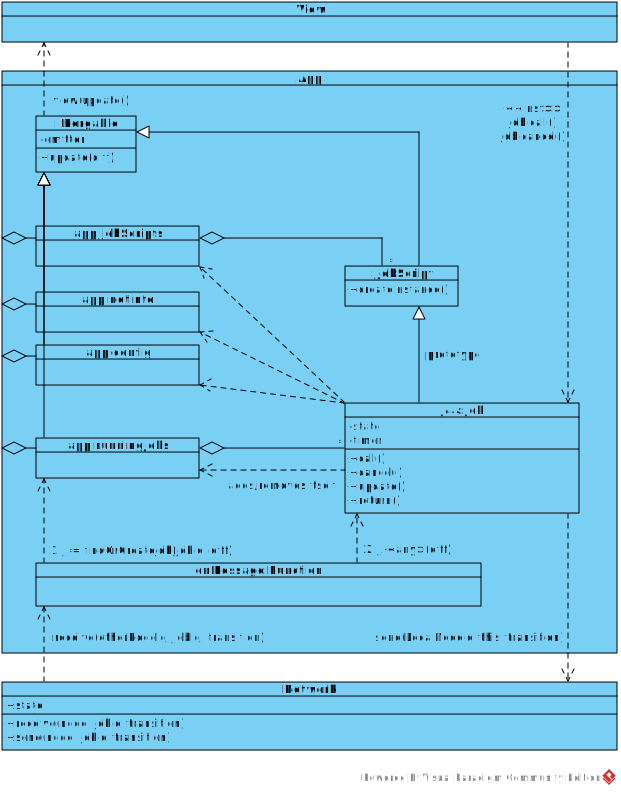
\includegraphics[width=0.9\textwidth]{vm}
  \end{center}
  \label{deploy}
  \label{viewModel}
  \caption{UML Object Diagramm des Client. Server and Worker enthalten keine View. }
\end{wrapfigure}
